\documentclass{beamer}
\mode<presentation>
\usepackage{amsmath}
\usepackage{amssymb}
%\usepackage{advdate}
\usepackage{adjustbox}
\usepackage{subcaption}
\usepackage{enumitem}
\usepackage{multicol}
\usepackage{listings}
\usepackage{url}
\def\UrlBreaks{\do\/\do-}
\usetheme{Boadilla}
\usecolortheme{lily}
\setbeamertemplate{footline}
{
  \leavevmode%
  \hbox{%
  \begin{beamercolorbox}[wd=\paperwidth,ht=2.25ex,dp=1ex,right]{author in head/foot}%
    \insertframenumber{} / \inserttotalframenumber\hspace*{2ex} 
  \end{beamercolorbox}}%
  \vskip0pt%
}
\setbeamertemplate{navigation symbols}{}

\providecommand{\nCr}[2]{\,^{#1}C_{#2}} % nCr
\providecommand{\nPr}[2]{\,^{#1}P_{#2}} % nPr
\providecommand{\mbf}{\mathbf}
\providecommand{\pr}[1]{\ensuremath{\Pr\left(#1\right)}}
\providecommand{\qfunc}[1]{\ensuremath{Q\left(#1\right)}}
\providecommand{\sbrak}[1]{\ensuremath{{}\left[#1\right]}}
\providecommand{\lsbrak}[1]{\ensuremath{{}\left[#1\right.}}
\providecommand{\rsbrak}[1]{\ensuremath{{}\left.#1\right]}}
\providecommand{\brak}[1]{\ensuremath{\left(#1\right)}}
\providecommand{\lbrak}[1]{\ensuremath{\left(#1\right.}}
\providecommand{\rbrak}[1]{\ensuremath{\left.#1\right)}}
\providecommand{\cbrak}[1]{\ensuremath{\left\{#1\right\}}}
\providecommand{\lcbrak}[1]{\ensuremath{\left\{#1\right.}}
\providecommand{\rcbrak}[1]{\ensuremath{\left.#1\right\}}}
\theoremstyle{remark}
\newtheorem{rem}{Remark}
\newcommand{\sgn}{\mathop{\mathrm{sgn}}}
\providecommand{\abs}[1]{\left\vert#1\right\vert}
\providecommand{\res}[1]{\Res\displaylimits_{#1}} 
\providecommand{\norm}[1]{\lVert#1\rVert}
\providecommand{\mtx}[1]{\mathbf{#1}}
\providecommand{\mean}[1]{E\left[ #1 \right]}
\providecommand{\fourier}{\overset{\mathcal{F}}{ \rightleftharpoons}}
%\providecommand{\hilbert}{\overset{\mathcal{H}}{ \rightleftharpoons}}
\providecommand{\system}{\overset{\mathcal{H}}{ \longleftrightarrow}}
	%\newcommand{\solution}[2]{\textbf{Solution:}{#1}}
%\newcommand{\solution}{\noindent \textbf{Solution: }}
\providecommand{\dec}[2]{\ensuremath{\overset{#1}{\underset{#2}{\gtrless}}}}
\newcommand{\myvec}[1]{\ensuremath{\begin{pmatrix}#1\end{pmatrix}}}
\let\vec\mathbf

\lstset{
%language=C,
frame=single, 
breaklines=true,
columns=fullflexible
}

\numberwithin{equation}{section}

\title{10.3.2.7}
\author{Prajwal \\ EE24BTECH11051}
\begin{document}

\begin{frame}
\titlepage
\end{frame}
\section*{Outline}
\begin{frame}
\tableofcontents
\end{frame}
\section{Problem}
\begin{frame}
\frametitle{Problem Statement}
Draw the graph of the equation $x − y + 1 = 0$ and $3x + 2y − 12 = 0$. Determine the coordinates of the vertices of the triangle formed by the lines and x-axis.
\end{frame}
%\subsection{Literature}
\section{Solution}
\subsection{Theoretical Solution}
\begin{frame}
\frametitle{Theoretical Solution}
Given,
\begin{align}
x-y+1=0\\
3x+2y-12=0\\
y=0
\end{align}
lines $x-y+1=0$ and $3x+2y-12=0$ touches `x-axis at,
\begin{align}
    x=-1\\
    x=4
\end{align}
Both given line touches at,
\begin{align}
    x=2\\
    y=3
\end{align}
\end{frame}
\section{Computational logic}
\begin{frame}[fragile]
    \frametitle{Computational logic}
	Let us assume the given system of equations are consistent and we will try solving using LU decomposition
	
	Given the system of linear equations:
	\begin{align}
	x-y+1=0\\
    3x+2y-12=0\\
    y=0
	\end{align}
	
	We rewrite the equations as:
	\begin{align}
		x_1 &= x, \\
        		x_2 &= y,
	\end{align}
	giving the system:
	\begin{align}
	x_1-x_2=-1\\
    3x_1+2x_2=12\\
    x_2=0
	\end{align}
\end{frame}
\begin{frame}[fragile]
 	\subsection*{Step 1: Convert to Matrix Form}
	We write the system as:
	\begin{align}
		A \mathbf{x} &= \mathbf{b},
	\end{align}
	where:
	\begin{align}
A_1 &= \begin{bmatrix} 1 & -1 \\ 0 & 1 \end{bmatrix},\\
A_2 &= \begin{bmatrix} 3 & 2 \\ 0 & 1 \end{bmatrix},\\
A_3 &= \begin{bmatrix} 1 & -1 \\ 3 & 2 \end{bmatrix},\\
\mathbf{x} &= \begin{bmatrix} x_1 \\ x_2 \end{bmatrix}, \\
\mathbf{b_1} &= \begin{bmatrix} -1 \\ 0 \end{bmatrix},\\
\mathbf{b_2} &= \begin{bmatrix} 12 \\ 0 \end{bmatrix},
\end{align}
\end{frame}
\begin{frame}[fragile]
    \begin{align}
        \mathbf{b_3} &= \begin{bmatrix} -1 \\ 12 \end{bmatrix}.
    \end{align}
    	\subsection*{Step 2: LU factorization using update equaitons}
    Given a matrix $ \mathbf{A} $ of size $ n \times n $, LU decomposition is performed row by row and column by column. The update equations are as follows:\\
    \textbf{LU decomposition by Doolittle's Method.}\\
1. Initialization: 
   - Start by initializing $ \mathbf{L} $ as the identity matrix $ \mathbf{L} = \mathbf{I} $ and $ \mathbf{U} $ as a copy of $ \mathbf{A} $.
   
2. Iterative Update:
   - For each pivot $ k = 1, 2, \ldots, n $:
     - Compute the entries of $ U $ using the first update equation.
     - Compute the entries of $ L $ using the second update equation.
        
\end{frame}
\begin{frame}[fragile]
 3. Result:
   - After completing the iterations, the matrix $ \mathbf{A} $ is decomposed into $ \mathbf{L} \cdot \mathbf{U} $, where $ \mathbf{L} $ is a lower triangular matrix with ones on the diagonal, and $ \mathbf{U} $ is an upper triangular matrix.
\subsection*{1. Update for $ U_{k,j} $ (Entries of $ U $)}

For each column $ j \geq k $, the entries of $ U $ in the $ k $-th row are updated as:
\[
U_{k,j} = A_{k,j} - \sum_{m=1}^{k-1} L_{k,m} \cdot U_{m,j}, \quad \text{for } j \geq k.
\]
This equation computes the elements of the upper triangular matrix $ \mathbf{U} $ by eliminating the lower triangular portion of the matrix.
\end{frame}
\begin{frame}[fragile]
    \subsection*{2. Update for $ L_{i,k} $ (Entries of $ L $)}

For each row $ i > k $, the entries of $ L $ in the $ k $-th column are updated as:
\[
L_{i,k} = \frac{1}{U_{k,k}} \left( A_{i,k} - \sum_{m=1}^{k-1} L_{i,m} \cdot U_{m,k} \right), \quad \text{for } i > k.
\]
This equation computes the elements of the lower triangular matrix $ \mathbf{L} $, where each entry in the column is determined by the values in the rows above it.\\
Using a code we get L,U as 
\begin{align}   
L_1 = \begin{bmatrix} 1 & 0 \\ 0 & 1 \end{bmatrix},
U_1 = \begin{bmatrix} 1 & -1 \\ 0 & 1 \end{bmatrix}\\
L_2 = \begin{bmatrix} 1 & 0 \\ 0 & 1 \end{bmatrix},
U_2 = \begin{bmatrix} 3 & 2 \\ 0 & 1 \end{bmatrix}\\
L_3 = \begin{bmatrix} 1 & 0 \\ 3 & 1 \end{bmatrix},
U_3 = \begin{bmatrix} 1 & -1 \\ 0 & 5 \end{bmatrix}
\end{align}
\end{frame}
\begin{frame}[fragile]
    	\subsection*{Step 3: Solve $L\mathbf{y} = \mathbf{b}$ (Forward Substitution)}
	We solve:
	\begin{align}
		L_1\mathbf{y_1} = \mathbf{b_1} \quad \text{or} \quad \begin{bmatrix} 1 & 0 \\ 0 & 1 \end{bmatrix} \begin{bmatrix} y_1 \\ y_2 \end{bmatrix} = \begin{bmatrix} -1 \\ 0 \end{bmatrix}.\\
        L_2\mathbf{y_2} = \mathbf{b_2} \quad \text{or} \quad \begin{bmatrix} 1 & 0 \\ 0 & 1 \end{bmatrix} \begin{bmatrix} y_1 \\ y_2 \end{bmatrix} = \begin{bmatrix} 12 \\ 0 \end{bmatrix}.\\
        L_3\mathbf{y_3} = \mathbf{b_3} \quad \text{or} \quad \begin{bmatrix} 1 & 0 \\ 3 & 1 \end{bmatrix} \begin{bmatrix} y_1 \\ y_2 \end{bmatrix} = \begin{bmatrix} -1 \\ 15 \end{bmatrix}.
	\end{align}
	Thus:
	\begin{align}
		\mathbf{y_1} &= \begin{bmatrix} -1 \\ 0 \end{bmatrix}.\\
        \mathbf{y_2} &= \begin{bmatrix} 12 \\ 0 \end{bmatrix}.\\
        \mathbf{y_3} &= \begin{bmatrix} -12 \\ 0 \end{bmatrix}.\\
	\end{align}
\end{frame}
\begin{frame}[fragile]
    	\subsection*{Step 4: Solve $U\mathbf{x} = \mathbf{y}$ (Backward Substitution)}
	We solve:
	\begin{align}
		U_1\mathbf{x_1} = \mathbf{y_1} \quad \text{or} \quad \begin{bmatrix} 1 & -1 \\ 0 & 1 \end{bmatrix} \begin{bmatrix} x_1 \\ x_2 \end{bmatrix} = \begin{bmatrix} -1 \\ 0 \end{bmatrix}.\\
        U_2\mathbf{x_2} = \mathbf{y_2} \quad \text{or} \quad \begin{bmatrix} 3 & 2 \\ 0 & 1 \end{bmatrix} \begin{bmatrix} x_1 \\ x_2 \end{bmatrix} = \begin{bmatrix} 12 \\ 0 \end{bmatrix}.\\
        U_3\mathbf{x_3} = \mathbf{y_3} \quad \text{or} \quad \begin{bmatrix} 1 & -1 \\ 0 & 5 \end{bmatrix} \begin{bmatrix} x_1 \\ x_2 \end{bmatrix} = \begin{bmatrix} -12 \\ 0 \end{bmatrix}.\\
	    \mathbf{x_1} &= \begin{bmatrix} -1 \\ 0 \end{bmatrix}.\\
        \mathbf{x_2} &= \begin{bmatrix} 4 \\ 0 \end{bmatrix}.\\
        \mathbf{x_3} &= \begin{bmatrix} 2 \\ 3 \end{bmatrix}.
	\end{align}
\end{frame}
\begin{frame}[fragile]
    \begin{figure}[h]
    \centering
    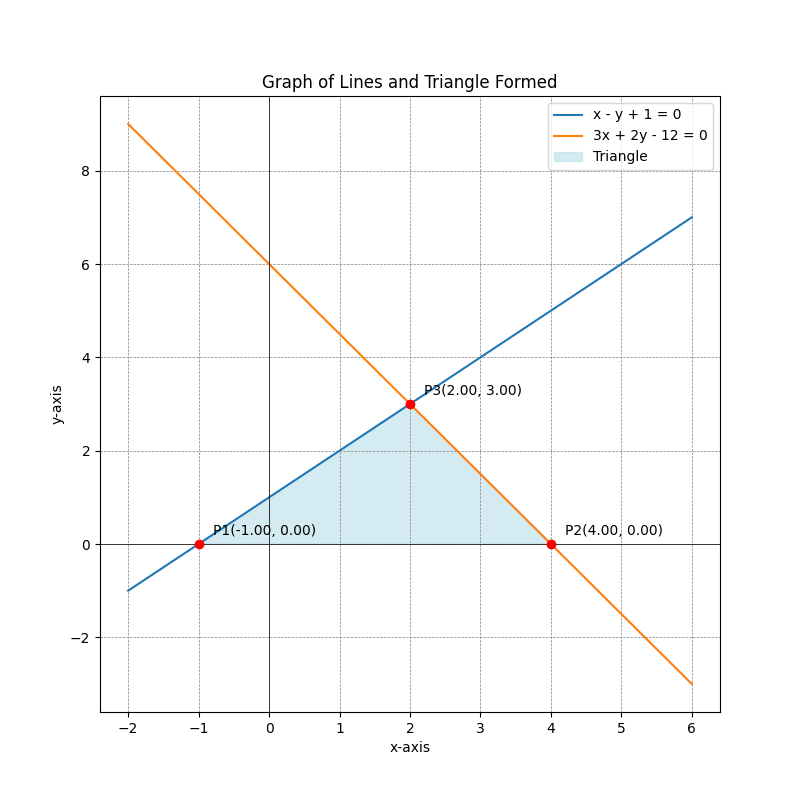
\includegraphics[width=\columnwidth]{figs/Figure_1.png}
 \end{figure}
\end{frame}
\end{document}
